\documentclass[border=10pt]{standalone}
\usepackage{xcolor}
\usepackage{pgfplots}
\usepackage{tikz}
\begin{document}
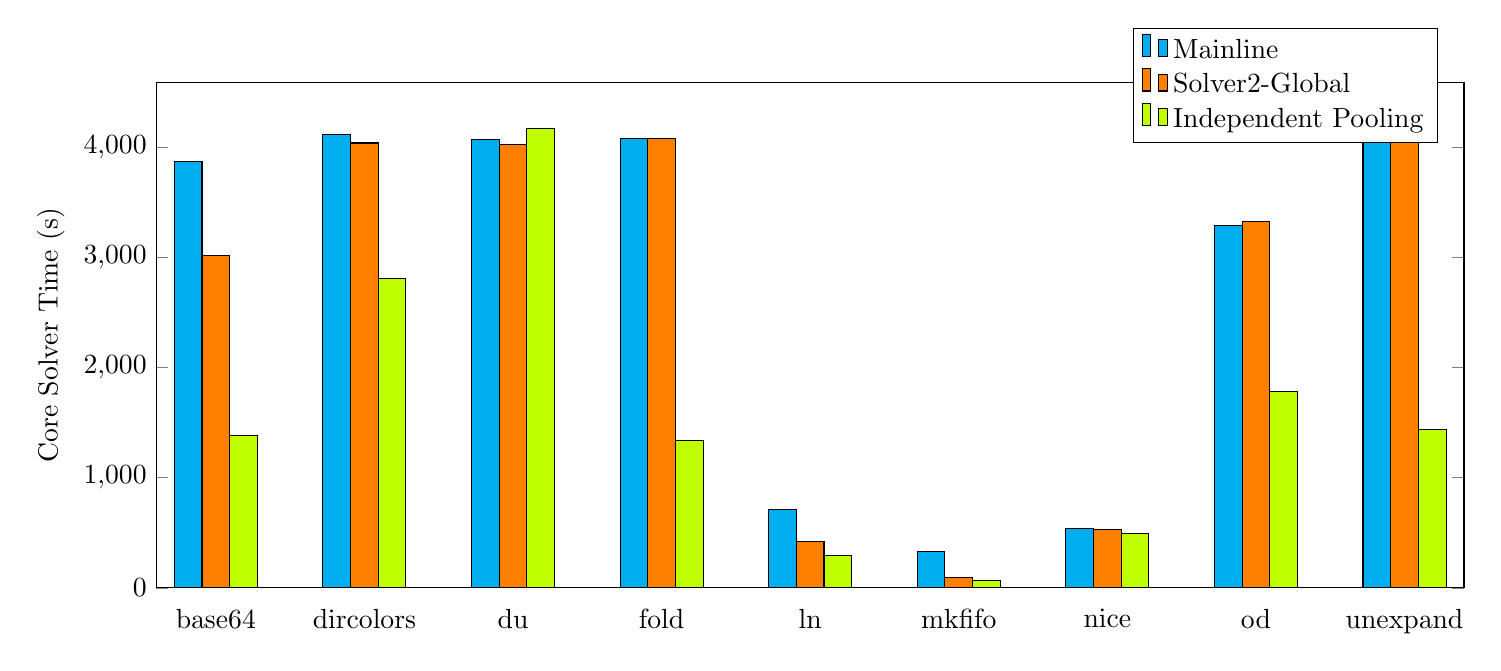
\begin{tikzpicture}
    \begin{axis}[
        width  = 1.5 * \textwidth,
        height = 8cm,
        major x tick style = transparent,
        % tickwidth=10,
        ybar=0,
        bar width=10pt,
        % ymajorgrids = true,
        ylabel = {Core Solver Time (s)},
        symbolic x coords={base64,dircolors,du,fold,ln,mkfifo,nice,od,unexpand},
        xtick = data,
        scaled y ticks = false,
        enlarge x limits=0.05,
        ymin=0,
        legend cell align=left,
        legend style={
                at={(0.98,0.88)},
                anchor=south east,
                % column sep=1ex
        }
    ]
        \addplot[style={cyan,fill=cyan,mark=none}, draw=black]
	coordinates {(base64,3865.22) (dircolors,4115.09) (du,4068.98) (fold,4079.20) (ln,712.81) (mkfifo,332.97) (nice,537.45) (od,3286.79) (unexpand,4098.55)};
\addplot[style={orange,fill=orange,mark=none}, draw=black]
	coordinates {(base64,3012.14) (dircolors,4035.77) (du,4022.94) (fold,4073.16) (ln,423.03) (mkfifo,92.94) (nice,530.53) (od,3323.00) (unexpand,4100.41)};
\addplot[style={lime,fill=lime,mark=none}, draw=black]
	coordinates {(base64,1381.28) (dircolors,2803.19) (du,4167.85) (fold,1339.10) (ln,296.19) (mkfifo,68.39) (nice,489.90) (od,1782.81) (unexpand,1433.44)};

        \legend{Mainline,Solver2-Global,Independent Pooling}
    \end{axis}
\end{tikzpicture}
\end{document}
